

% This is a simple sample document.  For more complicated documents take a look in the exercise tab. Note that everything that comes after a % symbol is treated as comment and ignored when the code is compiled.

\documentclass{article} % \documentclass{} is the first command in any LaTeX code.  It is used to define what kind of document you are creating such as an article or a book, and begins the document preamble

\usepackage{amsmath} % \usepackage is a command that allows you to add functionality to your LaTeX code
\usepackage{tikz}
\usepackage{enumitem}
\usepackage{varwidth}
\usepackage{tasks}
\usepackage[T1]{fontenc}

\usetikzlibrary{automata, positioning}

\newlength{\drop}
% The preamble ends with the command \begin{document}
\begin{document} % All begin commands must be paired with an end command somewhere
    \begin{titlepage}
        \drop=0.1\textheight
        \centering
        \vspace*{\baselineskip}
        {\LARGE Automata}\\[0.2\baselineskip]
        \rule{\textwidth}{0.4pt}\vspace*{-\baselineskip}\vspace{3.2pt}
        \rule{\textwidth}{1.6pt}\\[\baselineskip]
        \scshape
        Course Work 1.3\\
        F29LP\par
        \vfill
        Submitted by \\[\baselineskip]
        {\Large Yoav Levi\par}
        {\itshape H00347035\par}
        \vspace*{8\baselineskip}
    \end{titlepage}

    \section{/$(ab)*$/} % creates a section
    \section{/$(b*a)+a+b[ab]*$/}
    \section{NFA}
    \begin{enumerate}
        \item $L=\{w\in \{a,b\}\ast | \text{w contains at most two a's}\}$\\
            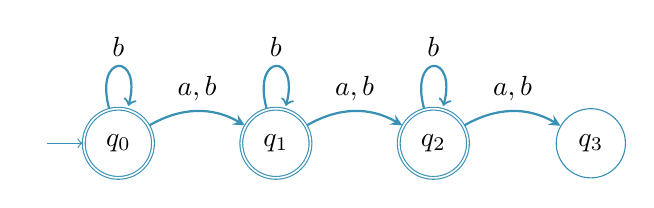
\begin{tikzpicture} [draw=cyan!70!black,
                node distance = 2cm, 
                on grid, 
                auto]
            
                % State q0 
                \node (q0) [state, 
                    initial, 
                    accepting, 
                    initial text = {}] {$q_0$};
                
                % State q1    
                \node (q1) [state,
                    accepting, 
                    right = of q0] {$q_1$};
                
                % State q2    
                \node (q2) [state,
                    accepting,
                    right = of q1] {$q_2$};
                
                % State q1    
                \node (q3) [state,
                    right = of q2] {$q_3$};
                
                % Arrows
                \path [-stealth, thick]
                    (q0) edge[bend left] node {$a,b$}   (q1)
                    (q1) edge[bend left] node {$a,b$}   (q2)
                    (q2) edge[bend left] node {$a,b$}   (q3)
                
                    (q0) edge [loop above]  node {$b$}()
                    (q1) edge [loop above]  node {$b$}()
                    (q2) edge [loop above]  node {$b$}();
            \end{tikzpicture}
        \item $L=\{w\in \{a,b\}\ast | \text{w contains an even number of occurrences of ab as a subword}\}$\\
            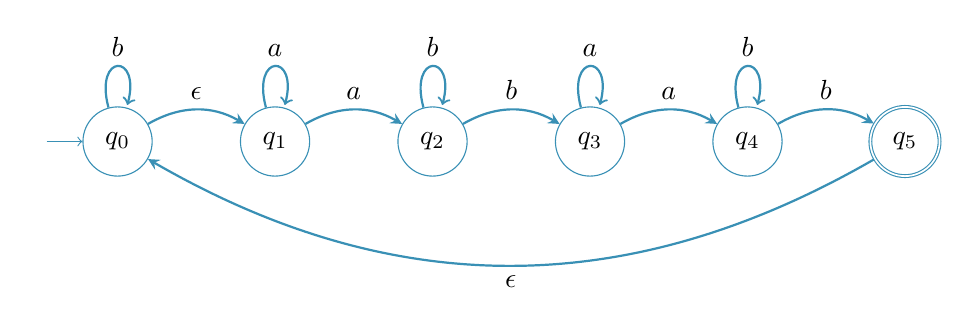
\begin{tikzpicture} [draw=cyan!70!black,
                node distance = 2cm, 
                on grid, 
                auto]
            
            % State q0 
            \node (q0) [state, 
                initial,  
                initial text = {}] {$q_0$};
            
            % State q1    
            \node (q1) [state, 
                right = of q0] {$q_1$};
            
            % State q2    
            \node (q2) [state,
                right = of q1] {$q_2$};
            
            % State q3    
            \node (q3) [state,
                right = of q2] {$q_3$};
            
            % State q4    
            \node (q4) [state,
                right = of q3] {$q_4$};

            % State q5
            \node (q5) [state,
                accepting,
                right = of q4] {$q_5$};
            
            % Arrows
            \path [-stealth, thick]
                (q0) edge[bend left] node {$\epsilon$}   (q1)
                (q1) edge[bend left] node {$a$}   (q2)
                (q2) edge[bend left] node {$b$}   (q3)
                (q3) edge[bend left] node {$a$}   (q4)
                (q4) edge[bend left] node {$b$}   (q5)
                (q5) edge [bend left]  node {$\epsilon$} (q0)
            
                (q0) edge [loop above]  node {$b$}()
                (q1) edge [loop above]  node {$a$}()
                (q2) edge [loop above]  node {$b$}()
                (q3) edge [loop above]  node {$a$}()
                (q4) edge [loop above]  node {$b$}();
            \end{tikzpicture}
        \item $L=\{w\in \{a,b\}\ast | \text{the first and the last letter of w are identical}\}$\\
            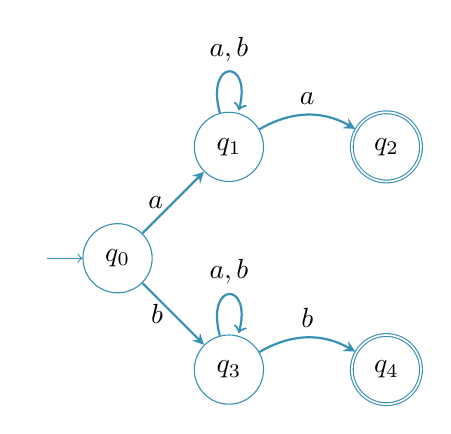
\begin{tikzpicture} [draw=cyan!70!black,
                node distance = 2cm, 
                on grid, 
                auto]
            
            % State q0 
            \node (q0) [state, 
                initial,  
                initial text = {}] {$q_0$};
            
            % State q1    
            \node (q1) [state, 
                above right = of q0] {$q_1$};
            
            % State q2    
            \node (q2) [state,
                accepting,
                right = of q1] {$q_2$};
            
            
            % State q1    
            \node (q3) [state, 
                below right = of q0] {$q_3$};
            
            % State q2    
            \node (q4) [state,
                accepting,
                right = of q3] {$q_4$};
            
            % Arrows
            \path [-stealth, thick]
                (q0) edge [left] node {$a$} (q1)
                (q0) edge [left] node {$b$} (q3)
                (q1) edge [bend left] node {$a$} (q2)
                (q3) edge [bend left] node {$b$} (q4)
            
                (q1) edge [loop above]  node {$a,b$}()
                (q3) edge [loop above]  node {$a,b$}()
                ;
            \end{tikzpicture}
    \end{enumerate}
    \section{/$a*(ba\{2,\})*$/}
    \section{}
            \begin{gather*}
                S \to aA\\
                A \to aB\\
                B \to aS | aC\\
                C \to aS | \epsilon
            \end{gather*}
    \section{Unmarked, N/A}
    \section{}
        \begin{enumerate}
            \item
            \begin{gather*}
                S \to aA | bB\\
                A \to aA | bS | aB | \epsilon\\
                B \to aS
            \end{gather*}
            \item Is ambiguous as "aaaa" can be constructed in two ways
            \begin{center}
                \begin{varwidth}{\textwidth}
                \begin{tasks}[label={(\Roman*)},label-width={1cm}] (2)
                    \task
                    \begin{tabular}{ c c}
                        Rule & Result\\
                        $S \to aA$ & a\\
                        $A \to aA$ & aa\\
                        $A \to aA$ & aaa\\
                        $A \to aA$ & aaaa\\
                        $A \to \epsilon$ & $\underline{aaaa}$
                    \end{tabular}

                    \task
                    \begin{tabular}{ c c}
                        Rule & Result\\
                        $S \to aA$ & a\\
                        $A \to aB$ & aa\\
                        $B \to aS$ & aaa\\
                        $S \to aA$ & aaaa\\
                        $A \to \epsilon$ & $\underline{aaaa}$
                    \end{tabular}
                \end{tasks}
                \end{varwidth}
            \end{center}
        \end{enumerate}
    \section{ The CFG is used to create a number of a's with an equivalent number of b's, in any order.}
    \section{$L=\{a^mb^na^m|m,n \geq 0\}$, alphabet = $\{a,b,Z_0\}$, Start stack symbol = $Z_0$}
        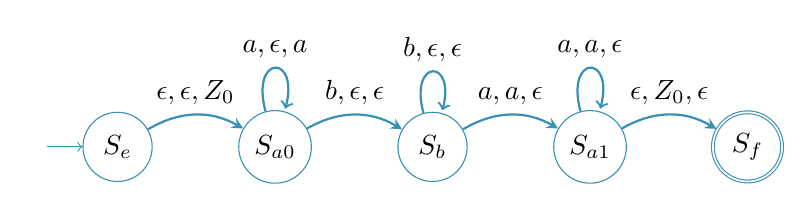
\begin{tikzpicture} [draw=cyan!70!black,
            node distance = 2cm, 
            on grid, 
            auto]
        
            % State q0 
            \node (se) [state, 
                initial, 
                initial text = {}] {$S_{e}$};

            % State q1    
            \node (sa0) [state,
                right = of se] {$S_{a0}$};

            % State q2    
            \node (sb) [state,
                right = of sa0] {$S_b$};

            % State q1    
            \node (sa1) [state,
                right = of sb] {$S_{a1}$};

            \node (sf) [state,
            accepting,
            right = of sa1] {$S_f$};

            % Arrows
            \path [-stealth, thick]
                (se) edge[bend left] node {$\epsilon,\epsilon,Z_0$}   (sa0)
                (sa0) edge[bend left] node {$b,\epsilon,\epsilon$}   (sb)
                (sb) edge[bend left] node {$a,a,\epsilon$}   (sa1)
                (sa1) edge[bend left] node {$\epsilon,Z_0,\epsilon$}   (sf)

                (sa0) edge [loop above]  node {$a,\epsilon,a$}()
                (sb) edge [loop above]  node {$b,\epsilon,\epsilon$}()
                (sa1) edge [loop above]  node {$a,a,\epsilon$}();
        \end{tikzpicture}
    \section{Not possible as DFA express regular languages, and $a^m b^n a^m$ is a only expressible as a context-free language.}
    \section{L=$\{a^m b^{2n}|m,n \geq 0\}$}
        \begin{tikzpicture} [draw=cyan!70!black,
            node distance = 3.5cm, 
            on grid, 
            auto]
        
            % State q0 
            \node (se) [state, 
                initial, 
                initial text = {}] {$S_{e}$};

            % State q1    
            \node (sa) [state,
                right = of se] {$S_{a}$};

            % State q2    
            \node (sb) [state,
                right = of sa0] {$S_b$};

            % State q1    
            \node (sf) [state,
                right = of sb] {$S_{f}$};

            % Arrows
            \path [-stealth, thick]
                (se) edge[bend left] node {$\epsilon,\epsilon,Z_0$}   (sa)
                (sa) edge[bend left] node {$b,\epsilon,b$}   (sb)
                (sa) edge[bend right] node {$\epsilon,\epsilon,\epsilon$}   (sb)
                (sb) edge[bend left] node {$b,\epsilon,b$}   (sa)
                (sb) edge[bend left] node {$\epsilon,Z_0,\epsilon$}   (sf)

                (sa) edge [loop above]  node {$a,\epsilon,\epsilon$}()
                ;
        \end{tikzpicture}
    \section{L=$\{a^mb^n|m>n>0\}$}
        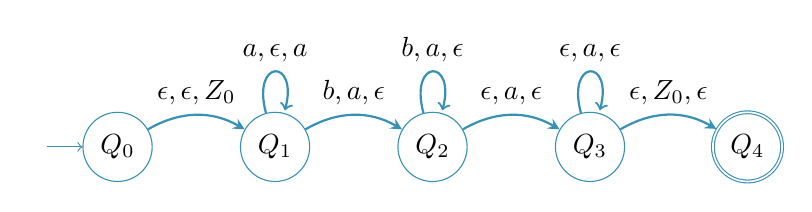
\begin{tikzpicture} [draw=cyan!70!black,
            node distance = 2cm, 
            on grid, 
            auto]
        
            % State q0 
            \node (q0) [state, 
                initial, 
                initial text = {}] {$Q_0$};

            % State q1    
            \node (q1) [state,
                right = of q0] {$Q_1$};

            % State q2    
            \node (q2) [state,
                right = of q1] {$Q_2$};

            % State q1    
            \node (q3) [state,
                right = of q2] {$Q_3$};

            \node (q4) [state,
            accepting,
            right = of q3] {$Q_4$};

            % Arrows
            \path [-stealth, thick]
                (q0) edge[bend left] node {$\epsilon,\epsilon,Z_0$}   (q1)
                (q1) edge[bend left] node {$b,a,\epsilon$}   (q2)
                (q2) edge[bend left] node {$\epsilon,a,\epsilon$}   (q3)
                (q3) edge[bend left] node {$\epsilon,Z_0,\epsilon$}   (q4)

                (q1) edge [loop above]  node {$a,\epsilon,a$}()
                (q2) edge [loop above]  node {$b,a,\epsilon$}()
                (q3) edge [loop above]  node {$\epsilon,a,\epsilon$}();
        \end{tikzpicture}
    \section{$L=\{W|\#_a W = \#_b W\}$}
        \begin{tikzpicture} [draw=cyan!70!black,
            node distance = 4cm, 
            on grid, 
            auto]
        
        % State S
        \node (s) [state, 
            initial,  
            initial text = {}] {$s$};

        % State q0 
        \node (q0) [state, 
            right = of s] {$q_0$};
        
        % State q1    
        \node (q1) [state, 
            above right = of q0] {$q_1$};

        % State q2   
        \node (q2) [state, 
         below right = of q0] {$q_2$};
        
        % State q3    
        \node (q3) [state,
            accepting,
            below right = of q1] {$q_3$};
        
        
        
        % Arrows
        \path [-stealth, thick]
            (s) edge [bend left] node {$\epsilon,\epsilon,Z_0$} (q0)
            (q0) edge [bend left] node {$b,\epsilon,b$} (q1)
            (q0) edge [bend right] node {$a,\epsilon,a$} (q2)
            (q1) edge [bend left] node {$\epsilon,Z_0,\epsilon$} (q3)
            (q2) edge [bend right ] node {$\epsilon,Z_0,\epsilon$} (q3)
        
            (q1) edge [loop above]  node {$a,b,\epsilon$}()
            (q1) edge [loop below]  node {$b,\epsilon,b$}()

            (q2) edge [loop above]  node {$b,a,\epsilon$}()
            (q2) edge [loop below]  node {$a,\epsilon,a$}()
            ;
        \end{tikzpicture}
    \section{L=$\{W|\#_a W=2\#_b W\}$}
        \begin{tikzpicture} [draw=cyan!70!black,
            node distance = 4cm, 
            on grid, 
            auto]
        
        % State S
        \node (s) [state, 
            initial,  
            initial text = {}] {$s$};

        % State q0 
        \node (q0) [state, 
            right = of s] {$q_0$};
        
        % State q1    
        \node (q1) [state, 
            above right = of q0] {$q_1$};

        % State q2   
        \node (q2) [state, 
         below right = of q0] {$q_2$};
        
        % State q3    
        \node (q3) [state,
            right = of q1] {$q_3$};
        
        % State q4    
        \node (q4) [state,
            right = of q2] {$q_4$};

        % State q5    
        \node (q5) [state,
            accepting,
            below right = of q3] {$q_5$};
        
        
        
        % Arrows
        \path [-stealth, thick]
            (s) edge [bend left] node {$\epsilon,\epsilon,Z_0$} (q0)
            (q0) edge [bend left] node {$b,\epsilon,b$} (q1)
            (q0) edge [bend right] node {$a,\epsilon,a$} (q2)
            (q1) edge [bend right] node {$\epsilon,\epsilon,b$} (q3)
            (q2) edge [bend left] node {$\epsilon,\epsilon,a$} (q4)
            (q4) edge [bend right] node {$\epsilon,Z_0,\epsilon$} (q5)
            (q3) edge [bend left ] node {$\epsilon,Z_0,\epsilon$} (q5)
        
            (q3) edge [loop above]  node {$a,b,\epsilon$}()
            (q3) edge [loop below]  node {$b,\epsilon,b$}()

            (q4) edge [loop above]  node {$b,a,\epsilon$}()
            (q4) edge [loop below]  node {$a,\epsilon,a$}()
            ;
        \end{tikzpicture}
    \section{}
        \begin{tikzpicture} [draw=cyan!70!black,
            node distance = 4cm, 
            on grid, 
            auto]
        
        % State S
        \node (s) [state, 
            initial,  
            initial text = {}] {$s$};

        % State q0 
        \node (q0) [state, 
            right = of s] {$q_0$};
        
        % State q1    
        \node (q1) [state,
            accepting,
            above right = of q0] {$q_1$};

        % State q2   
        \node (q2) [state, 
         accepting,
         below right = of q0] {$q_2$};
        
        % State q3    
        \node (q3) [state,
            below right = of q1] {$q_3$};
        
        
        
        % Arrows
        \path [-stealth, thick]
            (s) edge [bend left] node {$\epsilon,\epsilon,Z_0$} (q0)
            (q0) edge [bend left] node {$b,\epsilon,b$} (q1)
            (q0) edge [bend right] node {$a,\epsilon,a$} (q2)
            (q1) edge [bend left] node {$\epsilon,Z_0,\epsilon$} (q3)
            (q2) edge [bend right ] node {$\epsilon,Z_0,\epsilon$} (q3)
        
            (q1) edge [loop above]  node {$a,b,\epsilon$}()
            (q1) edge [loop below]  node {$b,\epsilon,b$}()

            (q2) edge [loop above]  node {$b,a,\epsilon$}()
            (q2) edge [loop below]  node {$a,\epsilon,a$}()
            ;
        \end{tikzpicture}
\end{document} % This is the end of the document
